\documentclass[12pt]{article}
\usepackage[letterpaper, margin=1in]{geometry}
\usepackage{graphicx}
\usepackage{subcaption}
\graphicspath{{./Figures/}}
\usepackage{hyperref}
\usepackage{parskip}
\usepackage{amsmath}
\usepackage{amssymb}
\usepackage{mathrsfs}
\usepackage{enumitem}
\usepackage{gensymb}
\allowdisplaybreaks

\title{ELECENG 3CL4 Lab 4 Pre-lab}
\author{
    Aaron Pinto \\
    pintoa9 \\
    L02
    \and
    Raeed Hassan \\
    hassam41 \\
    L02
}

\begin{document}

\maketitle
\clearpage

\section{Pre-lab Design Exercise}
\begin{enumerate}
	\item % q1
    For a second-order underdamped system with no zeros, the real part of a closed-loop pole can be approximated by $\frac{-4}{\text{settling time}}$. Therefore, we can approximate the real part of the desired closed-loop poles as $\frac{-4}{0.75} = -\frac{16}{3} = a$. Similarly, we can approximate $\zeta$ from the expression $\zeta = -\frac{\ln\left(\frac{P.O.}{100}\right)}{\sqrt{\pi^2 + \ln^2\left(\frac{P.O.}{100}\right)}}$. For our desired percent overshoot of 30\%, $\zeta = 0.3579$. Therefore, we know the angle of the pole from the negative real-axis is $\phi = \cos^{-1}(\zeta) = 1.2048$ rad or 69 degrees, and the imaginary part of the closed-loop pole must be $b = a\tan(\phi) = 2.6094a$. This means that we need a pole with a real part of less than $a = -\frac{16}{3}$ and an imaginary part of less than $2.6094a$.

    As these approximations are for a second-order system, we should place our poles a bit under the calculated values as we are dealing with a third-order system with a zero. For our closed-loop poles, we have chosen to place them at $-6 + 15j$ and $-6 - 15j$.

    \item % q2
    The root locus of the described system for $0 < k_c < +\infty$ is shown in Figure~\ref{fig:q2_root_locus}. As we can see, there are no values of $k_c$ that would allow us to place the closed-loop poles at $-6 + 15j$ or $-6 - 15j$.
    \begin{figure}[h]
        \centering
        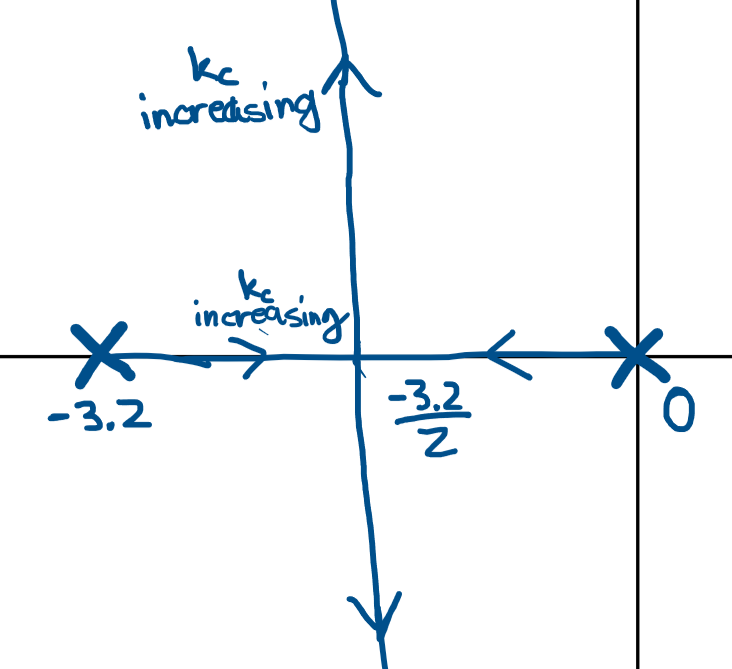
\includegraphics[width=0.5\textwidth]{q2}
        \caption{\label{fig:q2_root_locus}The Root Locus of the Closed-Loop Control System for Increasing $k_c$}
    \end{figure}

    \item % q3
    The angle of $G(s_0)$ is equal to the sum of the angle contributions of the two poles of $G(s)$ or $-\angle (s_0 - 0) - \angle (s_0 - (-3.2))$. For $s_0 = -6 + 15j$, we can calculate $\angle G(s_0) = -\angle (s_0 - 0) - \angle (s_0 - (-3.2)) = -111.80\degree - 100.57\degree = \angle G(s_0) = -212.37\degree$. We know from the phase condition that $\angle G(s_0) + \angle G_c(s_0) = 180\degree + l360\degree$, therefore the required angle contribution for the controller is equal to $\angle G_c(s_0) = 32.37\degree + l360\degree = \phi_c$. The phase lead compensator can help provide this required phase as it will provide us with a zero and a pole that we can adjust to meet the phase condition.

    \item % q4
    To begin, we will place the zero of the phase lead compensator $z$ right under the desired dominant closed-loop pole $s_0$, therefore $z = -6$. With the zero placed, the required angle contribution from the pole $p$ becomes $\angle (s_0 + p) = \angle (s_0 + z) - \phi_c  = 90\degree - 32.37\degree + l360\degree = 57.63\degree + l360\degree$. The position of $p$ can be calculated to be $p = z - \omega \tan(\phi_c) = -15.51$. Therefore, the values of $z$ and $p$ are $z = -6$ and $p = -15.51$.

    \item %q5
    The root locus of the system is shown in Figure~\ref{fig:q5_root_locus}. As we can see, the new root locus now places the desired closed-loop poles in the paths of the root locus.
    \begin{figure}[h]
        \centering
        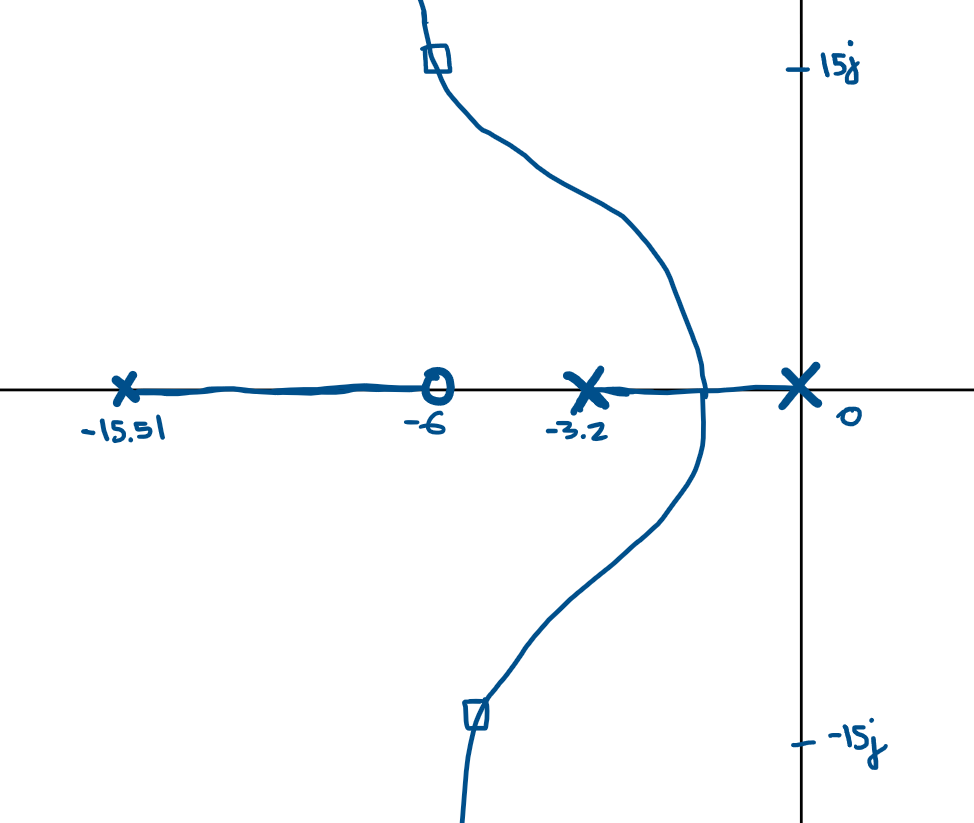
\includegraphics[width=0.5\textwidth]{q5}
        \caption{\label{fig:q5_root_locus}The Root Locus of the Closed-Loop Control System}
    \end{figure}

    \item %q6
    We can compute the value of $k_c$ that would place two of the closed-loop poles at the desired locations using the magnitude condition:
    \begin{equation*}
    \begin{aligned}
        1 &= |k_c k_G| \frac{\Pi |s_0 + z_i|}{\Pi |s_0 + p_j|} \\
        k_c k_G &= \frac{\Pi |s_0 + p_j|}{\Pi |s_0 + z_i|} \\
        k_c &= \frac{1}{k_G} \frac{\Pi |s_0 + p_j|}{\Pi |s_0 + z_i|} \\
        k_c &= \frac{1}{4.7} \frac{49.18}{15} \\
        k_c &= 0.6976
    \end{aligned}
    \end{equation*}

    \item %q7
    The closed-loop transfer function $T(s)$ is computed below:
    \begin{equation*}
    \begin{aligned}[b]
        G(s) &= \frac{4.7}{s(s + 3.2)} \\
        G_c(s) &= k_c\frac{s + z}{s + p} \\
        T(s) &= \frac{G(s)G_c(s)}{1 + G(s)G_c(s)} \\
        &= \frac{\frac{4.7 k_c (s + z)}{s(s + 3.2)(s + p)}}{1 + \frac{4.7 k_c (s + z)}{s(s + 3.2)(s + p)}} \\
        &= \frac{\frac{4.7 k_c (s + z)}{s(s + 3.2)(s + p)}}{\frac{s(s + 3.2)(s + p) + 4.7 k_c (s + z)}{s(s + 3.2)(s + p)}} \\
        &= \frac{4.7 k_c (s + z)}{s(s + 3.2)(s + p) + 4.7 k_c (s + z)} \\
        &= \frac{4.7 k_c (s + z)}{s^3 + ps^2 + 3.2s^2 + 3.2 p s + 4.7 k_c s + 4.7 k_c z} \\
        &= \frac{4.7 k_c (s + z)}{s^3 + (3.2 + p)s^2 + (3.2 p + 4.7 k_c)s + 4.7 k_c z} \\
        &= \frac{3.2787 (s - 6)}{s^3 - 12.31s^2 - 46.3533s - 19.6723} \\
    \end{aligned}
    \end{equation*}
    The form of the transfer function is a third-order system with 1 zero and 3 poles. We expect some deviation from the design objectives because we are doing all of our calculations based on approximations for a second-order system with no zeros, while the system we are designing has an extra pole and zero. We did pick values for our dominant poles that put them in safer positions to account for the extra pole and zero, but there may still be some deviation.

    \item % q8
    \begin{equation*}
    \begin{aligned}[b]
        k_v &= \lim_{s \to 0} \ sG_c(s)G(s) \\
        &= \lim_{s \to 0} \ s \frac{4.7 k_c (s + z)}{s(s + 3.2)(s + p)} \\
        &= \lim_{s \to 0} \ \frac{4.7 k_c (s + z)}{(s + 3.2)(s + p)} \\
        &= \frac{4.7 k_c (0 + z)}{(0 + 3.2)(0 + p)} \\
        &= \frac{4.7 k_c z}{3.2 p} \\
        &= 0.3964 \\
        e_{ss} &= \frac{1}{k_v} \\
        &= 2.522
    \end{aligned}
    \end{equation*}
\end{enumerate}

\end{document}